\let\negmedspace\undefined
\let\negthickspace\undefined
\documentclass[journal]{IEEEtran}
\usepackage[a5paper, margin=10mm, onecolumn]{geometry}
\usepackage{lmodern} % Ensure lmodern is loaded for pdflatex
\usepackage{tfrupee} % Include tfrupee package

\setlength{\headheight}{1cm} % Set the height of the header box
\setlength{\headsep}{0mm}     % Set the distance between the header box and the top of the text

% --- Assuming gvv-book and gvv packages define \solution, \brak, etc. ---
\usepackage{gvv-book}
\usepackage{gvv}
\usepackage{cite}
\usepackage{amsmath,amssymb,amsfonts,amsthm}
\usepackage{algorithmic}
\usepackage{graphicx}
\graphicspath{{./figs/}}
\usepackage{textcomp}
\usepackage{xcolor}
\usepackage{txfonts}
\usepackage{listings}
\usepackage{enumitem}
\usepackage{mathtools}
\usepackage{gensymb}
\usepackage{comment}
\usepackage[breaklinks=true]{hyperref}
\usepackage{tkz-euclide} 
\usepackage{listings}
\usepackage{gvv}                                        
\def\inputGnumericTable{}                    
\usepackage[latin1]{inputenc}                                
\usepackage{color}                                            
\usepackage{array}                                            
\usepackage{longtable}                                       
\usepackage{calc}                            
\usepackage{multirow}                                         
\usepackage{hhline}                                          
\usepackage{ifthen}                                           
\usepackage{lscape}
\usepackage{circuitikz}

\begin{document}
	
	\bibliographystyle{IEEEtran}
	\vspace{3cm}
	
	\title{4.3.32}
	\author{EE25BTECH11042 - Nipun Dasari}
	\maketitle
		
	\renewcommand{\thefigure}{\theenumi}
	\renewcommand{\thetable}{\theenumi}
	\setlength{\intextsep}{10pt} % Space between text and floats
	
	
	\numberwithin{equation}{enumi}
	\numberwithin{figure}{enumi}
	\renewcommand{\thetable}{\theenumi}
	
	\textbf{Question}:\\
	Find the slope of a line which cuts off intercepts of equal length on the axes is. Solve using matrices. \\ 
	\solution \\
	Consider normal form of a line:
	\begin{align}
		\vec{n}^\top\vec{x} = 1
	\end{align}
	Given that equal intercepts are cut off we get 2 cases:\\
	On substituting the intercepts in place of $\vec{x}$: \\
	\textbf{Case 1: The intercepts are equal \brak{b = a}}
	\begin{align}
		\implies  \vec{n}^\top\begin{myvec}{a \\ 0} \end{myvec} = 1 \label{0.2}\\
		\implies \vec{n}^\top\begin{myvec}{0 \\ a} \end{myvec} = 1 \label{0.3} \\
	\end{align}
	
		from \eqref{0.2} and from \eqref{0.3}
		\begin{align}
		\vec{n}^\top\begin{myvec}{a & 0 \\ 0 & a} \end{myvec} = \begin{myvec}{1 & 1} \end{myvec} \\
		\implies a\vec{n}^\top\begin{myvec}{1 & 0 \\ 0 & 1}\end{myvec} = \begin{myvec}{1 & 1} \end{myvec}\\
		\implies a\vec{n}^\top\vec{I} = \begin{myvec}{1 & 1} \end{myvec}
		\implies a\vec{n}^\top = \begin{myvec}{1 & 1} \end{myvec}
		\implies \vec{n} = \frac{1}{a}\begin{myvec}{1 \\ 1} \end{myvec}
		\end{align}
		Thus, direction vector $\vec{n} = \begin{myvec}{1 \\ 1}\end{myvec}$
		

	\textbf{Case 2: The intercepts are negatives of each other \brak{-b = a}}
	\begin{align}
		\implies  \vec{n}^\top\begin{myvec}{a \\ 0} \end{myvec} = 1 \label{0.5}\\
		\implies \vec{n}^\top\begin{myvec}{0 \\ -a} \end{myvec} =1\label{0.6} \\
	\end{align}
		By \eqref{0.5}, \eqref{0.6}:
		\begin{align}
		\vec{n}^\top\begin{myvec}{a & 0 \\ 0 & -a} \end{myvec} = \begin{myvec}{1 & 1} \end{myvec} \\
		\implies a\vec{n}^\top\begin{myvec}{1 & 0 \\ 0 & -1}\end{myvec} = \begin{myvec}{1 & 1} \end{myvec}
	\end{align}
	Let $\vec{A} = \begin{myvec}{1 & 0 \\ 0 & -1}\end{myvec}$\\
	For this matrix $\vec{A} = \vec{A}^{-1}$
	\begin{align}
		\implies a\vec{n}^\top = \begin{myvec}{1 & 1}\vec{A}^{-1} \end{myvec}
		\implies a\vec{n}^\top = \begin{myvec}{1 & 1}\vec{A}^{-1} \end{myvec}
		\implies \vec{n} = \frac{1}{a}\begin{myvec}{1 \\ -1} \end{myvec}
		\end{align}
		Thus, direction vector $\vec{n} = \begin{myvec}{1 \\ -1}\end{myvec}$
		The direction vector is given \brak{\text{in general}} by:
		\begin{align}
			\vec{m} = 	\begin{myvec}{1\\ m}\end{myvec} \text{  where $m$ is slope of given line }
		\end{align}		
			On comparing with the obtained direction vectors
	\begin{align}
		\therefore m = \pm1
	\end{align}	
	\begin{figure}[H]
		\centering
		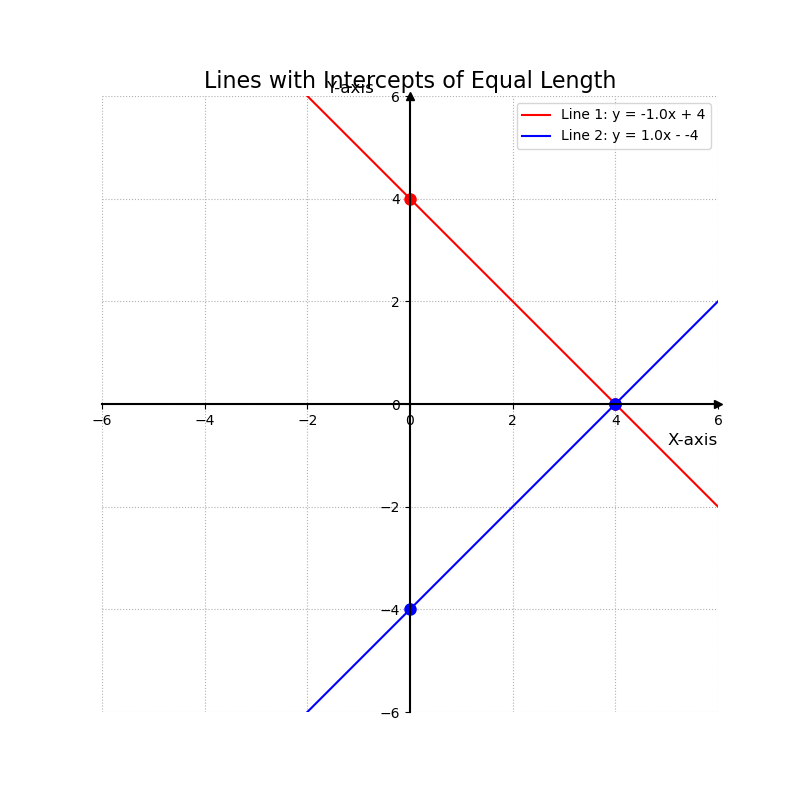
\includegraphics[width = 0.6\columnwidth]{Figure_1.png}
		\caption*{}
		\label{fig1}
	\end{figure}
	
\end{document}